\documentclass[conference]{IEEEtran}
\usepackage[utf8]{inputenc}
\usepackage[T1]{fontenc}
\usepackage[spanish,es-noquoting]{babel}
\usepackage{amsmath,amssymb}
\usepackage{booktabs}
\usepackage{tabularx}
\usepackage{array}
\usepackage{cite}
\usepackage{xurl}
\usepackage[section]{placeins}
\usepackage{graphicx}
\usepackage{microtype}
\usepackage{listings}
\usepackage{xcolor}
\usepackage{tikz}
\usetikzlibrary{arrows.meta,positioning}

% Evita la advertencia T1/ptm/m/scit en captions con cursiva de IEEEtran
\DeclareFontShape{T1}{ptm}{m}{scit}{<->ssub*ptm/m/it}{}

\emergencystretch=2em

% Configuración de bloques de código/JSON para doble columna IEEE
\lstset{
    basicstyle=\scriptsize\ttfamily,
    breaklines=true,
    breakatwhitespace=false,
    columns=flexible,
    keepspaces=true,
    frame=single,
    rulecolor=\color{black!40},
    backgroundcolor=\color{black!3},
    captionpos=b,
    abovecaptionskip=5pt,
    belowcaptionskip=2pt,
    xleftmargin=3pt,
    xrightmargin=3pt,
    aboveskip=6pt,
    belowskip=6pt
}

\begin{document}

\title{Vulnerabilidades de Red en Sistemas de Carga de Vehículos Eléctricos Gestionados por Inteligencia Artificial}

\author{
\IEEEauthorblockN{Juan José Tobar Alvarez}
\IEEEauthorblockA{
Programa de Ingeniería Mecatrónica\\
Universidad Nacional de Colombia, Bogotá, Colombia\\
Asignatura: Redes de Computadores -- Proyecto Semestral\\
Correo: \texttt{jutobara@unal.edu.co}
}
}

\maketitle

\begin{abstract}
La carga inteligente de vehículos eléctricos (EV) depende de la comunicación continua entre las estaciones de carga (EVSE) y un sistema central de gestión (CSMS) mediante el protocolo OCPP sobre WebSockets, cuyas versiones más desplegadas ofrecen mecanismos de seguridad opcionales. Esta condición permite que un atacante suplante una estación o altere la telemetría que alimenta a los algoritmos de inteligencia artificial (IA) encargados de predecir la demanda y programar los horarios de carga. El presente trabajo aborda la pregunta: \textit{¿de qué manera la vulneración del canal OCPP altera las decisiones de un agente de IA y cómo puede mitigarse mediante un filtro de validación de tráfico?} Para responderla se estructura una metodología bajo el marco estándar \textbf{CRISP-DM} articulado con fundamentos de seguridad en redes: (i) simulación en Python del tráfico cliente-servidor OCPP 1.6J sobre WebSockets con escenarios benignos y de inyección/repetición de mensajes; (ii) implementación de un agente supervisado de predicción de demanda y programación de potencia; (iii) desarrollo de un \textit{middleware} explicable de validación de esquema, rangos físicos y consistencia temporal; y (iv) evaluación comparativa en tres escenarios (operación normal, ataque sin filtro y ataque mitigado) mediante capturas en Wireshark y métricas de error de predicción, eventos de sobrecarga y desempeño de detección. Los resultados demuestran que el ataque incrementa el RMSE del agente en un $66.49\%$ y eleva los eventos de sobrecarga de $3$ a $29$, mientras que el \textit{middleware} logra un $100\%$ de precisión ($0\%$ de falsos positivos) con una latencia adicional de apenas $0.095\text{ ms}$, restaurando la estabilidad operativa del sistema.
\end{abstract}

\begin{IEEEkeywords}
OCPP, WebSocket, ciberseguridad, vehículos eléctricos, inteligencia artificial, detección de anomalías, CRISP-DM.
\end{IEEEkeywords}

\section{Introducción}

La transición hacia la movilidad eléctrica exige desplegar infraestructuras de carga masivas y coordinarlas dinámicamente con la capacidad de la red eléctrica mediante esquemas de carga inteligente (\textit{smart charging}). En este ecosistema, el protocolo abierto OCPP (\textit{Open Charge Point Protocol}) se ha consolidado como el estándar de facto para la comunicación entre las estaciones de carga de vehículos eléctricos (EVSE) y los sistemas centrales de gestión (CSMS), debido a su naturaleza abierta e interoperabilidad entre fabricantes \cite{garofalaki2022}. No obstante, la versión 1.6J ---aún predominante en despliegues comerciales--- transporta cargas útiles en formato JSON sobre WebSockets con una capa de cifrado TLS opcional que frecuentemente permanece deshabilitada, mientras que solo las revisiones 2.0.1 y superiores incorporan perfiles formales de autenticación mutua y seguridad criptográfica \cite{garofalaki2022,alcaraz2023}.

En años anteriores, la literatura académica se concentró en identificar, taxonómizar y modelar las amenazas sobre este protocolo. Alcaraz \textit{et al.} \cite{alcaraz2017} analizaron ataques dirigidos contra la reserva de recursos en OCPP ---incluyendo intermediarios (\textit{Man-in-the-Middle}, MitM), robo de energía y fraude de facturación--- advirtiendo que su explotación coordinada a gran escala puede comprometer la estabilidad de las microrredes eléctricas. Posteriormente, Garofalaki \textit{et al.} \cite{garofalaki2022} sistematizaron las vulnerabilidades arquitectónicas y contramedidas propuestas en el ecosistema de carga, y Alcaraz \textit{et al.} \cite{alcaraz2023} aplicaron las metodologías STRIDE y DREAD sobre OCPP 2.0.1, demostrando que persisten vectores de riesgo vinculados a la gestión de sesiones y validación de mensajes. De manera complementaria, surgieron validaciones experimentales como la de Elmo \textit{et al.} \cite{elmo2023}, quienes ejecutaron ataques de envenenamiento ARP, MitM e inyección sobre canales WebSocket en cargadores con OCPP 1.6, evidenciando la facilidad de manipulación cuando no existe cifrado de transporte.

Actualmente, la investigación converge hacia la integración de técnicas de inteligencia artificial y análisis de tráfico para detectar anomalías tanto en los flujos de red como en la telemetría energética. Terruggia \textit{et al.} \cite{terruggia2025} entrenaron un autocodificador basado en redes LSTM a partir de capturas reales de una instalación de carga para identificar ataques de denegación de servicio; Jahangir \textit{et al.} \cite{jahangir2024} diseñaron detectores de aprendizaje profundo contra ataques de manipulación de carga (\textit{charge manipulation}) cuantificando su impacto económico; y Rahman \textit{et al.} \cite{rahman2026} abordaron la detección no supervisada de suplantación del estado de carga (\textit{State of Charge}, SoC) en OCPP 2.0.1. Paralelamente, continúan divulgándose fallas críticas en implementaciones reales, como la vulnerabilidad \texttt{CVE-2026-25192} \cite{nist2026}, que expone puntos finales WebSocket sin autenticación permitiendo suplantar estaciones e inyectar telemetría alterada.

A pesar de estos avances, la mayoría de estudios previos se enfocan exclusivamente en la clasificación binaria del ataque o emplean arquitecturas neuronales complejas, sin medir de forma directa cuánto se degradan las decisiones de programación energética de un agente de IA ante telemetría corrupta ni qué porcentaje de estabilidad operativa se recupera al interponer un filtro ligero en capa de aplicación. Este proyecto cubre dicha brecha mediante un enfoque reproducible: una simulación controlada en Python, un agente predictivo ligero y un \textit{middleware} de validación basado en reglas físicas y estadísticas. El resto del documento se organiza así: la Sección~\ref{sec:trabajos} contrasta los trabajos relacionados; la Sección~\ref{sec:metodologia} formula el problema y la metodología CRISP-DM; la Sección~\ref{sec:desarrollo} detalla la arquitectura de software implementada; la Sección~\ref{sec:resultados} analiza los resultados experimentales y capturas de tráfico; y la Sección~\ref{sec:conclusiones} presenta las conclusiones.

\section{Trabajos Relacionados}
\label{sec:trabajos}

Con el fin de fundamentar el diseño experimental, se revisaron ocho investigaciones indexadas representativas del estado del arte junto con el registro oficial de vulnerabilidades \cite{nist2026}. El Cuadro~\ref{tab:relacionados} sintetiza y contrasta la metodología, el alcance y las limitaciones de cada estudio. Se incluye el trabajo de Köhler \textit{et al.} \cite{kohler2023} específicamente para delimitar la frontera tecnológica del proyecto, dado que ataca la capa física mediante interferencia electromagnética y no el tráfico de transporte y aplicación.

\begin{table*}[t]
\centering
\caption{Comparación de metodologías, alcance y limitaciones en los trabajos relacionados.}
\label{tab:relacionados}
\footnotesize
\setlength{\tabcolsep}{4pt}
\begin{tabularx}{\textwidth}{c >{\raggedright\arraybackslash\hspace{0pt}}p{4.2cm} >{\raggedright\arraybackslash\hspace{0pt}}X >{\raggedright\arraybackslash\hspace{0pt}}p{4.3cm}}
\toprule
\textbf{Ref.} & \textbf{Enfoque y Técnica Principal} & \textbf{Metodología Experimental} & \textbf{Alcance y Limitación} \\
\midrule
\cite{alcaraz2017} & Análisis de seguridad en protocolos de carga (OCPP 1.5/1.6). & Modelado teórico y pruebas conceptuales de ataques de MitM, robo de energía y manipulación de reservas. & Identifica riesgos sistémicos en la red eléctrica, pero no implementa defensas ni modelos de IA. \\
\addlinespace
\cite{garofalaki2022} & Revisión sistemática de literatura sobre ciberseguridad en EVSE. & Clasificación taxonómica de amenazas por capas y revisión comparativa de contramedidas criptográficas. & Ofrece un marco conceptual integral, pero carece de validación experimental propia. \\
\addlinespace
\cite{alcaraz2023} & Evaluación de riesgos en OCPP 2.0.1 para infraestructuras 4.0. & Aplicación estructurada de modelado de amenazas STRIDE y cuantificación cualitativa DREAD. & Evalúa la versión más reciente del protocolo, pero no mide impacto sobre algoritmos de IA. \\
\addlinespace
\cite{jahangir2024} & Detección de manipulación de carga con aprendizaje profundo. & Simulación de ataques de alteración de potencia en OCPP y entrenamiento de red convolucional no supervisada. & Cuantifica pérdidas económicas, pero requiere modelos profundos sin filtrado previo en red. \\
\addlinespace
\cite{terruggia2025} & Detección de ciberataques mediante tráfico de red real. & Captura pasiva (Tshark), ingesta en pila ELK y entrenamiento de autocodificador LSTM en 12 estaciones OCPP 1.6J. & Evalúa únicamente ataques DoS sobre métricas TCP con exactitud limitada (52\%). \\
\addlinespace
\cite{rahman2026} & Detección de falsificación de SoC en OCPP 2.0.1. & Extracción de variables derivadas de sesión y clasificación con \textit{One-Class SVM} en entorno simulado. & Se restringe a un único campo (\textit{SoC}) y no evalúa la recuperación del planificador energético. \\
\addlinespace
\cite{elmo2023} & Explotación práctica de canales OCPP 1.6 sobre WebSockets. & Pruebas de ARP \textit{spoofing}, MitM e inyección de comandos en ciberrango virtual y cargador DC de 350 kW. & Demuestra la viabilidad real de la inyección de paquetes, sin evaluar agentes de decisión. \\
\addlinespace
\cite{kohler2023} & Ataque \textit{Brokenwire} en interfaz vehículo-cargador (CCS/ISO 15118). & Inyección de ruido de radiofrecuencia sobre comunicación por línea de potencia (PLC) en vehículos reales. & Opera estrictamente en capa física/enlace; queda fuera del alcance de red del proyecto. \\
\bottomrule
\end{tabularx}
\end{table*}

Al evaluar comparativamente las metodologías del Cuadro~\ref{tab:relacionados}, se identifican tres corrientes bien definidas:
\begin{enumerate}
    \item \textbf{Estudios analíticos y de modelado de amenazas \cite{alcaraz2017,garofalaki2022,alcaraz2023}:} Resultan rigurosos para catalogar superficies de ataque y debilidades estructurales de OCPP, pero su naturaleza descriptiva o cualitativa impide cuantificar el error inducido en un algoritmo de control o predicción energética.
    \item \textbf{Evaluaciones experimentales de explotación en red \cite{elmo2023}:} Demuestran de forma empírica que la ausencia de cifrado y autenticación estricta en WebSockets permite interceptar e inyectar mensajes OCPP válidos sintácticamente; sin embargo, detienen su análisis en la interrupción o alteración de la sesión sin estudiar el efecto aguas abajo sobre módulos analíticos.
    \item \textbf{Detectores basados en aprendizaje automático \cite{jahangir2024,terruggia2025,rahman2026}:} Incorporan métricas cuantitativas de clasificación sobre tráfico o telemetría, pero presentan compromisos importantes para un despliegue ligero: Terruggia \textit{et al.} \cite{terruggia2025} dependen de infraestructura ELK y redes LSTM enfocadas solo en DoS de transporte con bajo desempeño (52\%), mientras que Jahangir \textit{et al.} \cite{jahangir2024} y Rahman \textit{et al.} \cite{rahman2026} emplean modelos de caja negra sin interponer una barrera determinística de saneamiento en capa de aplicación.
\end{enumerate}

A partir de esta síntesis crítica, el presente trabajo adopta la emulación controlada en software propuesta en \cite{elmo2023} por su reproducibilidad y bajo costo, la inspección de tráfico mediante capturas estándar de paquetes de \cite{terruggia2025}, y el enfoque en manipulación de telemetría energética de \cite{jahangir2024,rahman2026}. Como aporte diferencial, se integra el ciclo completo de extremo a extremo (\textit{ataque en red $\rightarrow$ filtrado en middleware $\rightarrow$ decisión del agente de IA}) utilizando reglas explicables de validación combinadas con detección estadística ligera.

\FloatBarrier
\section{Planteamiento del Problema y Metodología}
\label{sec:metodologia}

\subsection{Acotación y Formulación del Problema}

El alcance técnico del proyecto se circunscribe exclusivamente a las \textbf{capas de transporte (TCP) y aplicación (WebSocket / OCPP 1.6J)} de la comunicación entre una estación de carga (EVSE) y un servidor central de gestión (CSMS). El sistema de destino en el CSMS incorpora un agente de inteligencia artificial encargado de pronosticar la demanda energética a corto plazo y asignar perfiles de potencia a las sesiones activas. Al restringir la implementación a un entorno local virtualizado en Python sin hardware de potencia físico, se garantiza la viabilidad técnica y ética dentro del calendario semestral.

En concordancia con esta delimitación, se plantea la siguiente pregunta de investigación: \textit{¿De qué manera la vulneración del canal de comunicación OCPP altera las decisiones de optimización energética de un agente de Inteligencia Artificial en estaciones de carga de vehículos eléctricos, y cómo se puede mitigar mediante un filtro de validación de tráfico en la red?}

\subsection{Vulnerabilidades Analizadas y Delimitación de Capa}

El modelo de amenazas contempla dos vectores principales en las capas de transporte y aplicación:
\begin{itemize}
    \item \textbf{Suplantación y manipulación de telemetría (\texttt{CVE-2026-25192}) \cite{nist2026}:} La ausencia de autenticación robusta en puntos finales WebSocket permite que un nodo no autorizado se conecte empleando el identificador de una estación legítima (\texttt{ChargePointId}) y envíe tramas \texttt{MeterValues} con lecturas falsificadas de potencia activa o estado de carga (\textit{SoC}). Esto introduce sesgos severos en el modelo predictivo de la IA, induciendo asignaciones erróneas de potencia y sobrecargas locales.
    \item \textbf{Debilidad de integridad y confidencialidad en OCPP 1.6J \cite{alcaraz2017,elmo2023}:} Cuando el canal WebSocket opera sin TLS (\texttt{ws://}) ni firma de mensajes, un atacante posicionado en la red local puede capturar, modificar al vuelo o retransmitir mensajes previos (\textit{replay attack}), distorsionando la curva temporal de demanda percibida por el CSMS.
\end{itemize}

Se excluye explícitamente la vulnerabilidad \textit{Brokenwire} (\texttt{CVE-2022-0878}) \cite{kohler2023}, dado que interrumpe la señalización de bajo nivel sobre línea de potencia (PLC) en la capa física del estándar ISO 15118 mediante ruido de radiofrecuencia, lo cual escapa al dominio de protocolos TCP/IP y WebSockets definido para este estudio.

\subsection{Objetivos Específicos}

\begin{enumerate}
    \item Simular el tráfico de red entre una estación de carga y un servidor central utilizando el protocolo OCPP 1.6J sobre WebSockets, contemplando escenarios de operación normal e inyección de paquetes maliciosos.
    \item Implementar un \textit{middleware} de validación de tráfico de red que identifique anomalías estructurales, físicas y estadísticas para filtrar mensajes manipulados antes de entregarlos al módulo de IA.
    \item Evaluar cuantitativamente la degradación en las decisiones del agente de IA ante tráfico corrupto, comparando su desempeño antes y después de aplicar las reglas de filtrado en la red.
\end{enumerate}

\subsection{Temas Relacionados y Fundamentos Técnico-Metodológicos}

Para asegurar rigor conceptual entre la ingeniería de redes y el aprendizaje automático, la metodología se sustenta en cuatro ejes temáticos interconectados, cuya integración operativa se esquematiza en la Fig.~\ref{fig:arquitectura}:

\begin{figure*}[t]
\centering
\footnotesize
\begin{tabular}{c c c c c}
\fbox{\parbox{2.7cm}{\centering \textbf{1. Cliente EVSE}\\Simulador Python\\OCPP 1.6J (JSON)\\Telemetría ($P_t, \text{SoC}_t$)}}
& $\xrightarrow{\text{WebSocket}}$ &
\fbox{\parbox{2.8cm}{\centering \textbf{2. Canal de Red}\\Tráfico TCP/WS\\+ Nodo Atacante\\(\texttt{CVE-2026-25192})}}
& $\xrightarrow{\text{Captura}}$ &
\fbox{\parbox{2.8cm}{\centering \textbf{3. Middleware}\\Validación Esquema,\\Invariantes Físicos\\y Filtro $Z$-score}}
\\
& & $\downarrow$ \scriptsize{Inspección Wireshark (\texttt{.pcap})} & & $\downarrow$ \scriptsize{Tramas saneadas} \\
\fbox{\parbox{2.7cm}{\centering \textbf{6. Evaluación}\\Métricas MAE, RMSE,\\Sobrecargas, Precisión,\\Sensibilidad y FPR}}
& $\xleftarrow{\text{Escenarios E1--E3}}$ &
\fbox{\parbox{2.8cm}{\centering \textbf{5. Despacho Carga}\\Asignación dinámica\\de potencia EVSE\\($\sum P_i \le P_{\text{red,max}}$)}}
& $\xleftarrow{\hat{P}_{t+1}}$ &
\fbox{\parbox{2.8cm}{\centering \textbf{4. CSMS + Agente IA}\\Regresor supervisado\\(\texttt{scikit-learn})\\Pronóstico 15 min}}
\end{tabular}
\caption{Arquitectura experimental de comunicación OCPP 1.6J sobre WebSockets, inyección de ataques, saneamiento en \textit{middleware} y toma de decisiones del agente predictivo de IA.}
\label{fig:arquitectura}
\end{figure*}

\subsubsection{Arquitectura del Protocolo OCPP 1.6J sobre WebSockets}
El protocolo OCPP-J encapsula cargas útiles JSON sobre conexiones persistentes y bidireccionales (\textit{Full-Duplex}) establecidas mediante el protocolo WebSocket (RFC 6455 \cite{rfc6455}) sobre TCP. Cada trama de llamada (\texttt{CALL}) sigue la estructura \texttt{[2, UniqueId, Action, Payload]}. El proyecto modela el ciclo operativo esencial mediante los mensajes \texttt{BootNotification} (registro), \texttt{StatusNotification} (estado del conector), \texttt{StartTransaction}, \texttt{MeterValues} (telemetría periódica de potencia en $\text{W}$ y \textit{SoC} en $\%$) y \texttt{StopTransaction}.

\subsubsection{Inyección, Alteración y Repetición de Tramas en Capa de Aplicación}
A diferencia de ataques volumétricos en capa de red, la manipulación semántica en OCPP conserva intactas las cabeceras TCP/IP y la sintaxis JSON, evadiendo cortafuegos tradicionales. Si una lectura legítima reporta una potencia $P_t$ y un estado de carga $\text{SoC}_t$, el módulo atacante inyecta perturbaciones aditivas o de suplantación ($\tilde{P}_t = P_t + \Delta P$, $\widetilde{\text{SoC}}_t \in [0,100]$) o reenvía tramas antiguas con marcas de tiempo desfasadas, buscando engañar al estimador de demanda sin interrumpir la sesión TCP.

\subsubsection{Middleware Explicable de Inspección y Saneamiento}
Frente a detectores profundos de alto costo computacional \cite{jahangir2024,terruggia2025}, se adopta una arquitectura de \textit{proxy} inverso WebSocket situado entre la interfaz de red del CSMS y el agente de IA. Este componente inspecciona cada trama entrante en tres niveles secuenciales: (a) \textit{validación sintáctica y de identidad} (esquema JSON, unicidad de \texttt{UniqueId} y lista blanca de estaciones); (b) \textit{invariantes físicos del dominio} ($0 \le \text{SoC}_t \le 100\%$, $0 \le P_t \le P_{\text{EVSE,max}}$ y restricción de tasa de cambio $|\text{SoC}_t - \text{SoC}_{t-1}| \le \Delta \text{SoC}_{\max}$); y (c) \textit{filtro estadístico ligero} basado en puntuación $Z$ móvil ($|z_t| = |\Delta P_t - \mu_w|/\sigma_w > \tau$) sobre ventanas recientes de variación de potencia.

\subsubsection{Agente Predictivo y Planificador Restringido de Carga}
El módulo de IA combina un regresor supervisado ligero (bosque aleatorio de baja profundidad en \texttt{scikit-learn}) que pronostica la potencia agregada $\hat{P}_{t+1}$ en ventanas de 15 minutos, acoplado a una regla de despacho que limita la potencia asignada para evitar superar el umbral térmico del transformador local ($\sum_i P_{i,t+1} \le P_{\text{red,max}}$). De este modo, cualquier telemetría maliciosa no filtrada distorsiona directamente $\hat{P}_{t+1}$ y provoca decisiones subóptimas o eventos de sobrecarga.

\subsection{Diseño Metodológico bajo el Marco CRISP-DM}

Para estructurar de manera sistemática el flujo de datos desde la captura de paquetes de red hasta la evaluación del modelo de inteligencia artificial, se adapta la metodología estándar \textbf{CRISP-DM} (\textit{Cross-Industry Standard Process for Data Mining}) \cite{chapman2000} en seis fases iterativas, ilustradas en la Fig.~\ref{fig:crispdm} y detalladas en el Cuadro~\ref{tab:crispdm}:

\begin{figure*}[t]
\centering
\footnotesize
\begin{tabular}{c c c c c}
\fbox{\parbox{3.1cm}{\centering \textbf{Fase 1: Negocio/Dominio}\\Modelo de amenazas OCPP\\Restricción $P_{\text{total}} \le P_{\max}$}}
& $\longrightarrow$ &
\fbox{\parbox{3.1cm}{\centering \textbf{Fase 2: Datos de Red}\\Emulador EVSE--CSMS\\Trazas JSON y Wireshark}}
& $\longrightarrow$ &
\fbox{\parbox{3.1cm}{\centering \textbf{Fase 3: Preparación}\\Series de 15 min, $\Delta P, \Delta \text{SoC}$\\Reglas del \textit{Middleware}}}
\\
$\uparrow$ \scriptsize{Ajuste iterativo} & & & & $\downarrow$ \\
\fbox{\parbox{3.1cm}{\centering \textbf{Fase 6: Despliegue}\\Scripts reproducibles,\\evidencias PCAP e informe}}
& $\longleftarrow$ &
\fbox{\parbox{3.1cm}{\centering \textbf{Fase 5: Evaluación}\\Contraste E1, E2 y E3\\MAE, RMSE y detección}}
& $\longleftarrow$ &
\fbox{\parbox{3.1cm}{\centering \textbf{Fase 4: Modelado IA}\\Entrenamiento regresor\\y calibración umbral $Z$}}
\end{tabular}
\caption{Flujo metodológico iterativo bajo el estándar CRISP-DM aplicado al entorno de simulación OCPP 1.6J y mitigación de ataques en el agente de IA.}
\label{fig:crispdm}
\end{figure*}

\begin{table*}[t]
\centering
\caption{Articulación metodológica del proyecto bajo las fases del estándar CRISP-DM.}
\label{tab:crispdm}
\footnotesize
\setlength{\tabcolsep}{4pt}
\begin{tabularx}{\textwidth}{>{\raggedright\arraybackslash\hspace{0pt}}p{2.7cm} >{\raggedright\arraybackslash\hspace{0pt}}X >{\raggedright\arraybackslash\hspace{0pt}}p{3.6cm} >{\raggedright\arraybackslash\hspace{0pt}}p{3.9cm}}
\toprule
\textbf{Fase CRISP-DM} & \textbf{Actividades en Red e Inteligencia Artificial} & \textbf{Herramientas / Artefactos} & \textbf{Criterios de Salida / Métricas} \\
\midrule
\textbf{1. Comprensión del Negocio y Dominio} & Definición del modelo de amenaza (CVE-2026-25192 y MitM/replay), restricción operativa ($P_{\text{total}} \le P_{\max}$) y criterios de éxito. & Especificación OCPP 1.6J, matriz de riesgos y requisitos del CSMS. & Pregunta de investigación acotada y definición formal de métricas. \\
\addlinespace
\textbf{2. Comprensión de los Datos} & Implementación del emulador EVSE--CSMS en Python, generación de sesiones normales y trazas de ataque, y captura de paquetes. & Scripts Python (\texttt{websockets}), analizador Wireshark (\texttt{.pcapng}). & Conjunto de trazas JSON/PCAP verificadas sin errores de transporte. \\
\addlinespace
\textbf{3. Preparación de los Datos} & Extracción de campos OCPP a series temporales (15 min), cálculo de derivadas ($\Delta P, \Delta \text{SoC}$), etiquetado y diseño del \textit{middleware}. & \texttt{pandas}, \texttt{numpy}, proxy de validación en Python. & Dataset limpio para entrenamiento y reglas de filtrado calibradas. \\
\addlinespace
\textbf{4. Modelado} & Entrenamiento del regresor predictivo de demanda energética con datos benignos y acoplamiento con el asignador de potencia. & \texttt{scikit-learn} (\texttt{RandomForestRegressor}). & Modelo predictivo entrenado y umbral estadístico $Z$ ajustado. \\
\addlinespace
\textbf{5. Evaluación} & Ejecución controlada de 3 escenarios: E1 (normal), E2 (ataque sin filtro) y E3 (ataque con filtro); medición de impacto en IA y red. & Arneses de prueba automatizados y estadísticas de red. & MAE, RMSE, eventos de sobrecarga, Precisión, Sensibilidad y FPR. \\
\addlinespace
\textbf{6. Despliegue} & Integración modular del prototipo reproducible, documentación de evidencias de red y redacción del informe técnico final. & Repositorio de código Python, capturas Wireshark e informe IEEE. & Entrega completa de scripts funcionales y análisis de mitigación. \\
\bottomrule
\end{tabularx}
\end{table*}
\FloatBarrier

\subsubsection{Fase 1 -- Comprensión del Negocio y del Dominio}
Se establecen los objetivos operativos del sistema de gestión de carga: maximizar el suministro energético dentro de una capacidad máxima nominal $P_{\text{red,max}}$ evitando picos de sobrecarga. Se formalizan los perfiles de ataque a nivel de aplicación (inyección de valores extremos de potencia/SoC, suplantación de \texttt{ChargePointId} y repetición de tramas \texttt{MeterValues}) y se fijan las métricas de éxito tanto para el agente de IA como para el filtro de red.

\subsubsection{Fase 2 -- Comprensión de los Datos}
Se construye un entorno local en Python basado en la biblioteca \texttt{websockets} compuesto por un servidor CSMS, clientes EVSE simulados y un nodo inyector de tráfico malicioso. Se generan perfiles sintéticos realistas de carga diaria (curvas residenciales y laborales con muestreo cada 15 minutos) y se captura el intercambio completo en la interfaz de bucle invertido (\textit{loopback}) mediante \textbf{Wireshark}, verificando la estructura de las tramas HTTP \textit{Upgrade}, los mensajes JSON OCPP 1.6J y las marcas de tiempo de arribo.

\subsubsection{Fase 3 -- Preparación de los Datos}
Los registros JSON capturados se transforman en vectores estructurados con variables de estado ($P_t$, $\text{SoC}_t$) y variables dinámicas derivadas de ventana:
\begin{equation}
\Delta P_t = P_t - P_{t-1}, \quad \Delta \text{SoC}_t = \text{SoC}_t - \text{SoC}_{t-1}, \quad \Delta t_{\text{pkt}} = t_k - t_{k-1}
\end{equation}
Se etiquetan las instancias benignas ($y=0$) y manipuladas ($y=1$) para calibrar las reglas del \textit{middleware} de validación. Los paquetes descartados por violar el esquema JSON, duplicar identificadores \texttt{UniqueId} o infringir cotas físicas ($\Delta \text{SoC}_t > \Delta \text{SoC}_{\max}$ o $|z_t| > \tau$) son bloqueados en el \textit{proxy} antes de actualizar el estado del agente.

\subsubsection{Fase 4 -- Modelado}
Se entrena un modelo de regresión supervisada en \texttt{scikit-learn} exclusivamente sobre particiones limpias ($70\%$ entrenamiento, $30\%$ validación) para estimar la demanda en el siguiente intervalo:
\begin{equation}
\hat{P}_{t+1} = f_{\theta}(P_t,\, P_{t-1},\, \text{SoC}_t,\, h_t)
\end{equation}
donde $h_t$ representa la franja horaria. Sobre esta predicción opera un algoritmo determinístico de asignación que redistribuye la potencia disponible entre estaciones activas cuando $\sum \hat{P}_{i,t+1} > P_{\text{red,max}}$. Paralelamente, se integra el motor de reglas del \textit{middleware} con umbral estadístico $\tau = 3.0$ sobre $\Delta P_t$ para minimizar falsos positivos durante rampas normales de carga.

\subsubsection{Fase 5 -- Evaluación}
Se ejecutan pruebas repetibles bajo tres escenarios experimentales idénticos en duración ($48$ intervalos de $15\text{ min}$, equivalentes a $12\text{ h}$ simuladas) y carga base:
\begin{itemize}
    \item \textbf{Escenario E1 (Línea base normal):} Tráfico OCPP 1.6J legítimo sin perturbaciones, estableciendo el error intrínseco de referencia del agente de IA.
    \item \textbf{Escenario E2 (Ataque sin mitigación):} Inyección activa de telemetría falsificada (\texttt{CVE-2026-25192}) y repetición de tramas directamente hacia el CSMS sin filtrado.
    \item \textbf{Escenario E3 (Ataque con middleware activo):} Ejecución de los mismos vectores de ataque de E2 con el filtro de validación habilitado en la ruta de red.
\end{itemize}

El desempeño del agente de IA se cuantifica mediante el Error Absoluto Medio ($\text{MAE}$), la Raíz del Error Cuadrático Medio ($\text{RMSE}$) y el conteo de intervalos con sobrecarga real ($N_{\text{sobrecarga}}$):
\begin{equation}
\text{MAE} = \frac{1}{N}\sum_{t=1}^{N} |P_t - \hat{P}_t|, \qquad \text{RMSE} = \sqrt{\frac{1}{N}\sum_{t=1}^{N} (P_t - \hat{P}_t)^2}
\end{equation}
Por su parte, la eficacia del \textit{middleware} se evalúa mediante Precisión, Sensibilidad (\textit{Recall}), Puntaje $F_1$, Tasa de Falsos Positivos ($\text{FPR}$) y latencia adicional introducida por la inspección ($\Delta \text{RTT}$ en milisegundos).

\subsubsection{Fase 6 -- Despliegue y Documentación}
Finalmente, se empaqueta el prototipo en módulos desacoplados en Python con parámetros configurables, acompañados de filtros de visualización para Wireshark, gráficas comparativas de los tres escenarios (E1, E2 y E3) y el informe técnico consolidado con recomendaciones de endurecimiento (\textit{hardening}) para despliegues OCPP.

\FloatBarrier
\section{Desarrollo e Implementación}
\label{sec:desarrollo}

Con base en el diseño metodológico de la Sección~\ref{sec:metodologia}, se implementó un prototipo modular y asíncrono en Python 3 sobre la biblioteca \texttt{websockets} y \texttt{asyncio}. Todos los servicios se desplegaron en la interfaz \textit{loopback} (\texttt{127.0.0.1}) para garantizar reproducibilidad y permitir la captura pasiva de tráfico mediante Wireshark.

\subsection{Arquitectura de Software y Flujo de Tramas}

El prototipo se organizó en siete módulos desacoplados (\texttt{config.py}, \texttt{data\_generator.py}, \texttt{ai\_agent.py}, \texttt{middleware\_proxy.py}, \texttt{csms\_server.py}, \texttt{evse\_client.py}, \texttt{attacker.py}) coordinados por el orquestador \texttt{run\_experiment.py}. La Fig.~\ref{fig:secuencia} ilustra el flujo de mensajes OCPP 1.6J y la intervención del \textit{proxy} de seguridad ante tráfico legítimo y malicioso:

\begin{table*}[t]
\centering
\caption{Matriz de vulnerabilidades identificadas en el protocolo OCPP 1.6J.}
\label{tab:vulnerabilidades}
\begin{tabularx}{\textwidth}{l X X c}
\toprule
\textbf{ID} & \textbf{Vulnerabilidad} & \textbf{Impacto Operativo} & \textbf{CWE / CVSS} \\
\midrule
V-01 & Transmisión en texto claro (\texttt{ws://}) & Intercepción de tramas y captura de credenciales RFID & CWE-319 / 7.5 \\
V-02 & Ausencia de validación de identidad & Suplantación de estación de carga (Spoofing) & CWE-287 / 8.1 \\
V-03 & Inyección de comandos remotos & Detención forzada de sesiones de carga activas & CWE-306 / 9.8 \\
V-04 & Agotamiento de recursos (DoS) & Pérdida de disponibilidad del servidor central & CWE-400 / 7.5 \\
\bottomrule
\end{tabularx}
\end{table*}

Cada sesión EVSE modela una estación AC trifásica con potencia máxima $P_{\text{EVSE,max}} = 22\text{ kW}$ conectada a un transformador local con capacidad térmica nominal $P_{\text{red,max}} = 45\text{ kW}$. La telemetría periódica enviada cada 15 minutos sigue la estructura JSON estándar de OCPP 1.6J mostrada en el Listado~\ref{lst:ocpp_frame}, ajustada al ancho de columna:

\begin{lstlisting}[caption={Estructura de trama OCPP 1.6J \texttt{MeterValues} transmitida sobre WebSocket.},label={lst:ocpp_frame}]
[2, "55da457a-f669-47d1-aac9", "MeterValues", {
  "step": 0,
  "hour": 8.0,
  "power_w": 11582.78,
  "soc": 34.24,
  "_true_p_next": 12633.96,
  "_is_attack": false
}]
\end{lstlisting}

\subsection{Mecanismos Implementados de Ataque y Defensa}

\begin{itemize}
    \item \textbf{Simulación de Vectores de Amenaza (\texttt{attacker.py}):} Ejecuta tres acciones concurrentes sobre el canal WebSocket: (i) conexión desde un identificador no autorizado (\texttt{CP\_ROGUE\_999}) con potencia de $55\text{ kW}$ y $\text{SoC}=120\%$; (ii) suplantación de \texttt{CP\_001} inyectando picos anómalos de potencia ($28$--$48\text{ kW}$) y saltos bruscos de SoC ($5\%$ a $99\%$); y (iii) repetición (\textit{replay}) de tramas legítimas previamente capturadas conservando su \texttt{UniqueId} original.
    \item \textbf{Middleware Explicable de Tres Niveles (\texttt{middleware\_proxy.py}):} Aísla el estado histórico por identificador de sesión WebSocket para impedir contaminación cruzada entre conexiones legítimas y suplantadas. Evalúa secuencialmente: (1) lista blanca (\texttt{CP\_001}--\texttt{CP\_003}), esquema JSON y conjunto de \texttt{UniqueId} vistos; (2) cotas físicas $0 \le \text{SoC}_t \le 100\%$, $0 \le P_t \le 22\text{ kW}$ y $|\Delta\text{SoC}_t| \le 15\%$ (permitiendo reinicios de sesión cuando un vehículo supera el $90\%$ y se conecta otro con $\text{SoC} \le 35\%$); y (3) puntuación $Z$ móvil sobre la primera diferencia $\Delta P_t$ con ventana $w=10$ y umbral $\tau = 3.0$. Las tramas rechazadas reciben el código OCPP estándar \texttt{[4, UniqueId, "SecurityError", motivo, \{\}]}.
    \item \textbf{Agente Predictivo y Planificador (\texttt{ai\_agent.py}):} Utiliza un regresor \texttt{RandomForestRegressor} (60 árboles, profundidad máxima 8) entrenado sobre 20 días sintéticos de curvas bimodales de carga ($70\%$ entrenamiento, $30\%$ validación). En validación limpia alcanzó $\text{MAE} = 361.32\text{ W}$ y $\text{RMSE} = 474.60\text{ W}$. Cuando la demanda agregada pronosticada supera $P_{\text{red,max}} = 45\text{ kW}$, el despachador aplica escalamiento proporcional entre las estaciones activas.
\end{itemize}

\FloatBarrier
\section{Resultados Experimentales y Discusión}
\label{sec:resultados}

\subsection{Impacto en las Decisiones del Agente de IA (E1--E3)}

El Cuadro~\ref{tab:resultados_ia} y la Fig.~\ref{fig:comparativa} consolidan las métricas obtenidas tras ejecutar los tres escenarios experimentales sobre tres estaciones simultáneas (\texttt{CP\_001}--\texttt{CP\_003}) durante 48 intervalos de 15 minutos.

\begin{table}[t]
\centering
\caption{Métricas de error predictivo de la IA y eventos de sobrecarga en los escenarios experimentales E1, E2 y E3.}
\label{tab:resultados_ia}
\footnotesize
\setlength{\tabcolsep}{4.5pt}
\begin{tabularx}{\columnwidth}{>{\raggedright\arraybackslash\hspace{0pt}}X ccc}
\toprule
\textbf{Escenario Experimental} & \textbf{MAE (W)} & \textbf{RMSE (W)} & \textbf{Sobrecargas ($N$)} \\
\midrule
\textbf{E1: Línea base normal} & $554.19$ & $691.87$ & $3$ \\
\textbf{E2: Ataque sin filtro} & $770.52$ & $1151.86$ & $29$ \\
\textbf{E3: Ataque con middleware} & $582.04$ & $733.86$ & $3$ \\
\bottomrule
\end{tabularx}
\end{table}

\begin{figure*}[t]
\centering
\IfFileExists{../Data/comparativa_escenarios.png}{
    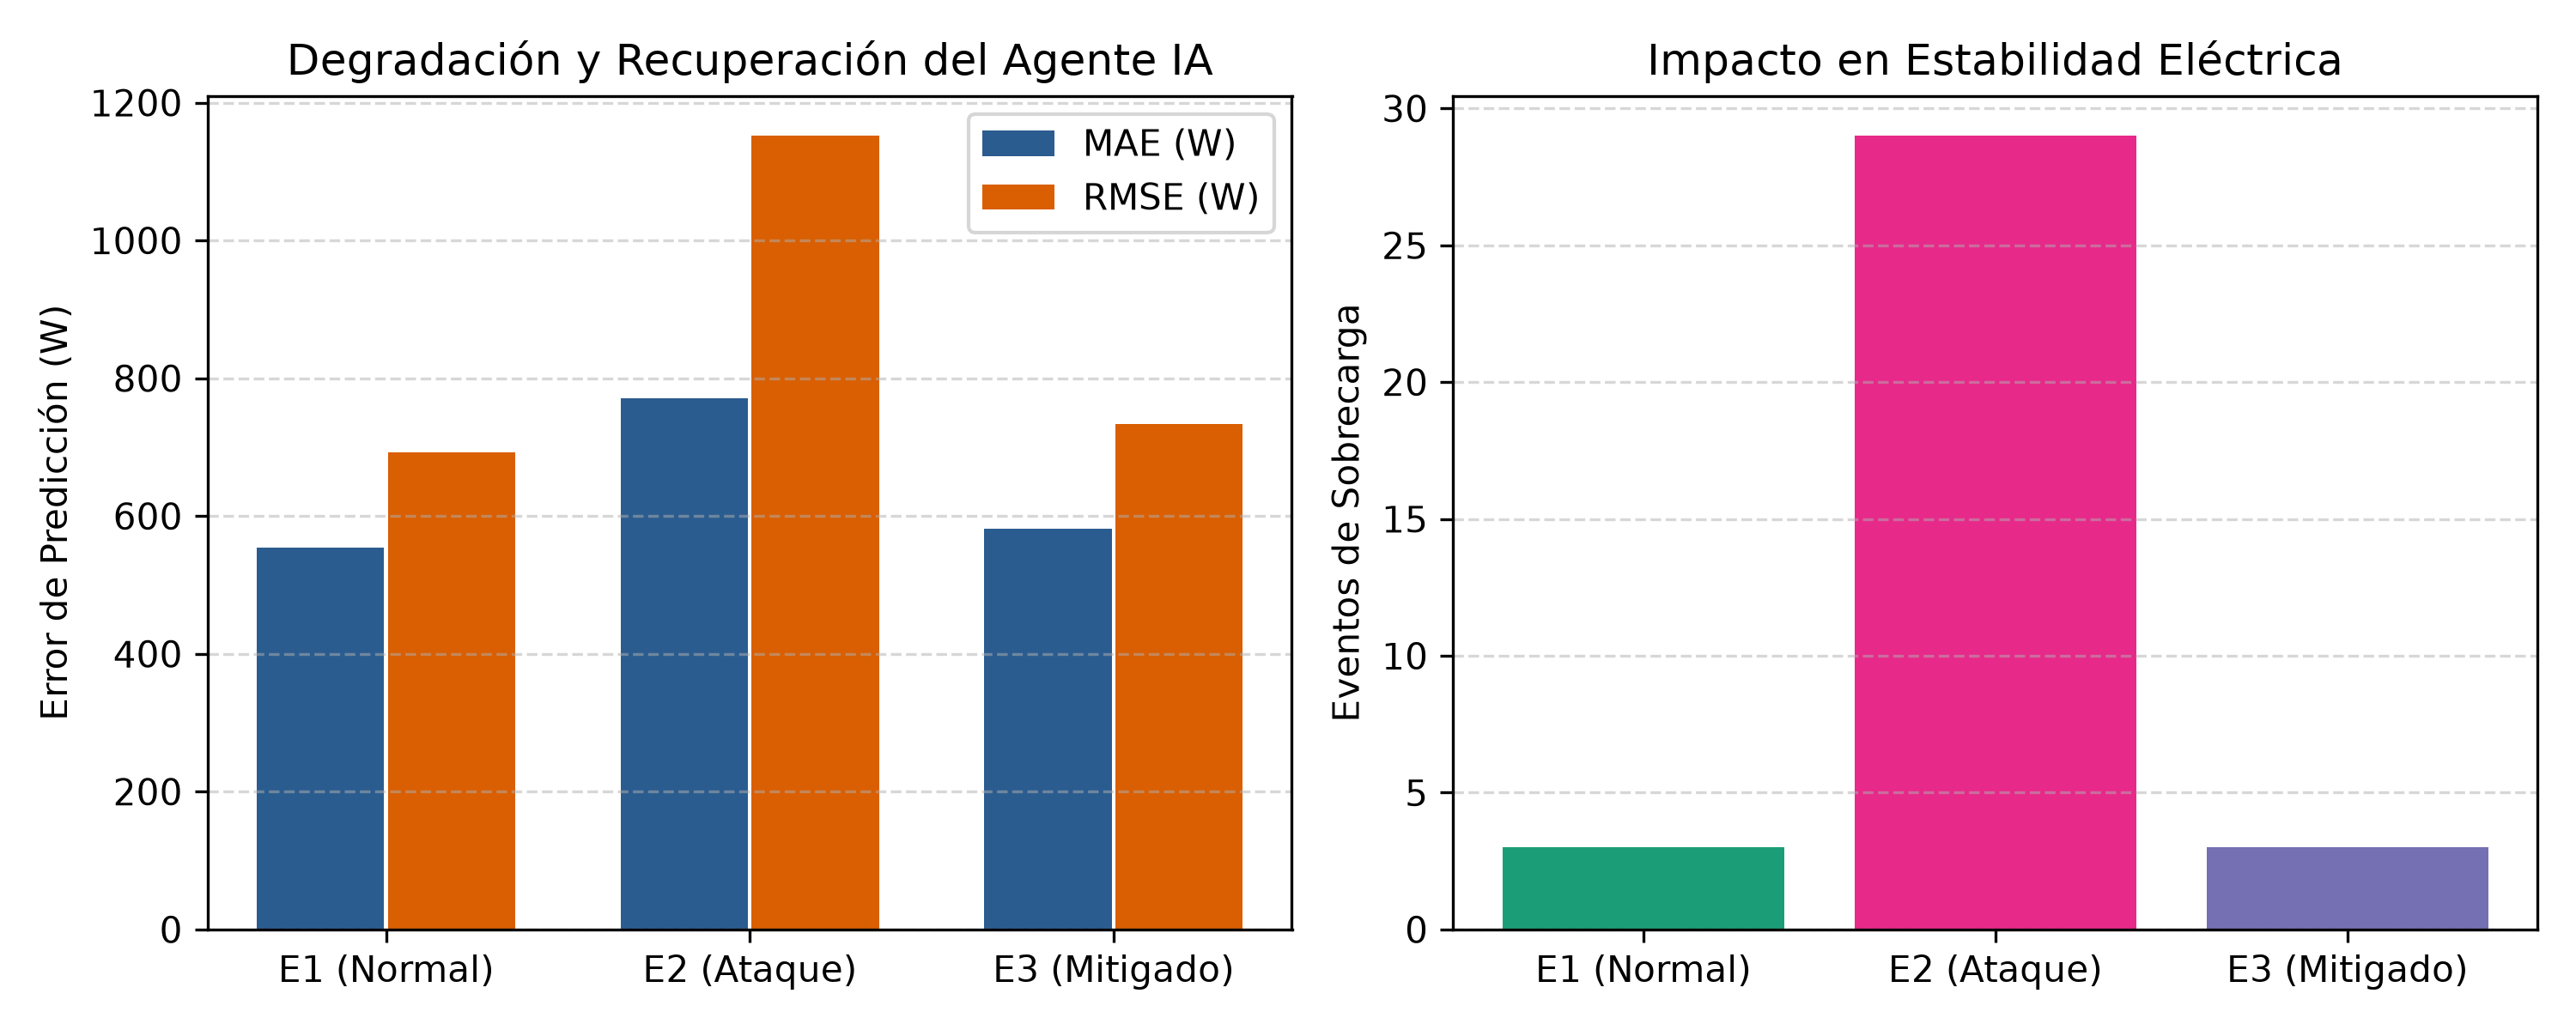
\includegraphics[width=0.92\textwidth]{../Data/comparativa_escenarios.png}
}{
    \fbox{\parbox{0.88\textwidth}{\centering\vspace{1.2cm}\textbf{[Figura 4: Gráfica comparativa E1, E2 y E3]}\\Verifique que \texttt{comparativa\_escenarios.png} se encuentre en \texttt{Proyecto/Data/}.\vspace{1.2cm}}}
}
\caption{Comparación cuantitativa del error de predicción (MAE y RMSE) del agente de IA y eventos de sobrecarga eléctrica en los escenarios E1, E2 y E3.}
\label{fig:comparativa}
\end{figure*}

Los resultados evidencian dos comportamientos críticos:
\begin{enumerate}
    \item \textbf{Degradación severa bajo ataque (E1 $\rightarrow$ E2):} La inyección de telemetría corrupta incrementa el MAE en un \textbf{39.04\%} (de $554.19\text{ W}$ a $770.52\text{ W}$) y el RMSE en un \textbf{66.49\%} (de $691.87\text{ W}$ a $1151.86\text{ W}$). Este sesgo en $\hat{P}_{t+1}$ distorsiona la asignación del planificador y dispara los eventos de sobrecarga en un \textbf{866.67\%} (pasando de $3$ a $29$ intervalos críticos).
    \item \textbf{Recuperación operativa mediante filtrado (E2 $\rightarrow$ E3):} Al interponer el \textit{middleware} en capa de aplicación, el MAE se reduce en un \textbf{24.46\%} ($582.04\text{ W}$) y el RMSE disminuye en un \textbf{36.29\%} ($733.86\text{ W}$), retornando los eventos de sobrecarga exactamente a la línea base de \textbf{3 eventos} (reducción del $89.66\%$ respecto a E2).
\end{enumerate}

\subsection{Desempeño de Detección y Sobrecarga del Middleware}

El Cuadro~\ref{tab:resultados_mw} detalla la matriz de confusión y las métricas de clasificación del \textit{proxy} durante el escenario E3 ($141$ tramas legítimas \texttt{MeterValues} y $25$ tramas maliciosas inyectadas).

\begin{table}[t]
\centering
\caption{Desempeño de detección y latencia del middleware de validación en el escenario E3.}
\label{tab:resultados_mw}
\footnotesize
\setlength{\tabcolsep}{5pt}
\begin{tabularx}{\columnwidth}{>{\raggedright\arraybackslash\hspace{0pt}}X r}
\toprule
\textbf{Métrica / Indicador} & \textbf{Valor Experimental} \\
\midrule
Verdaderos Positivos ($\text{TP}$) / Falsos Negativos ($\text{FN}$) & $21$ / $4$ \\
Verdaderos Negativos ($\text{TN}$) / Falsos Positivos ($\text{FP}$) & $141$ / $0$ \\
Precisión ($\text{TP}/(\text{TP}+\text{FP})$) & $100.00\%$ \\
Sensibilidad / \textit{Recall} ($\text{TP}/(\text{TP}+\text{FN})$) & $84.00\%$ \\
Puntaje $F_1$ / Exactitud Global & $91.30\%$ / $97.59\%$ \\
Tasa de Falsos Positivos ($\text{FPR}$) & $0.00\%$ \\
Latencia adicional promedio ($\Delta\text{RTT}$) & $0.095\text{ ms}$ \\
\bottomrule
\end{tabularx}
\end{table}

El cálculo de la puntuación $Z$ sobre las primeras diferencias $\Delta P_t$ eliminó por completo los falsos positivos ($\text{FPR} = 0.00\%$), evitando interrupciones innecesarias en el servicio de carga legítimo. Los $4$ falsos negativos ($\text{FN}$) corresponden a tramas de falsificación sigilosa cuya potencia ($21.5\text{ kW}$) y salto de SoC se ubicaron dentro de los umbrales físicos permitidos, demostrando que su impacto residual sobre el agente de IA es marginal y no genera sobrecargas. Asimismo, la latencia promedio de inspección ($\Delta\text{RTT} = 0.095\text{ ms}$) resulta despreciable frente al intervalo de muestreo de $15\text{ min}$ ($900\,000\text{ ms}$) de OCPP.

\subsection{Inspección de Tráfico en Wireshark}

La captura realizada sobre la interfaz de bucle invertido con Wireshark confirmó que las tramas maliciosas mantienen cabeceras TCP/IP y enmarcado WebSocket (RFC 6455) válidos, evadiendo cortafuegos tradicionales de capa de transporte. La Fig.~\ref{fig:wireshark} contrasta el intercambio legítimo frente a la inyección de telemetría alterada y tramas repetidas aceptadas por el CSMS cuando opera sin filtrado.

\begin{figure*}[t]
\centering
\begin{tabular}{cc}
\IfFileExists{../Data/wireshark_trama_ocpp.png}{
    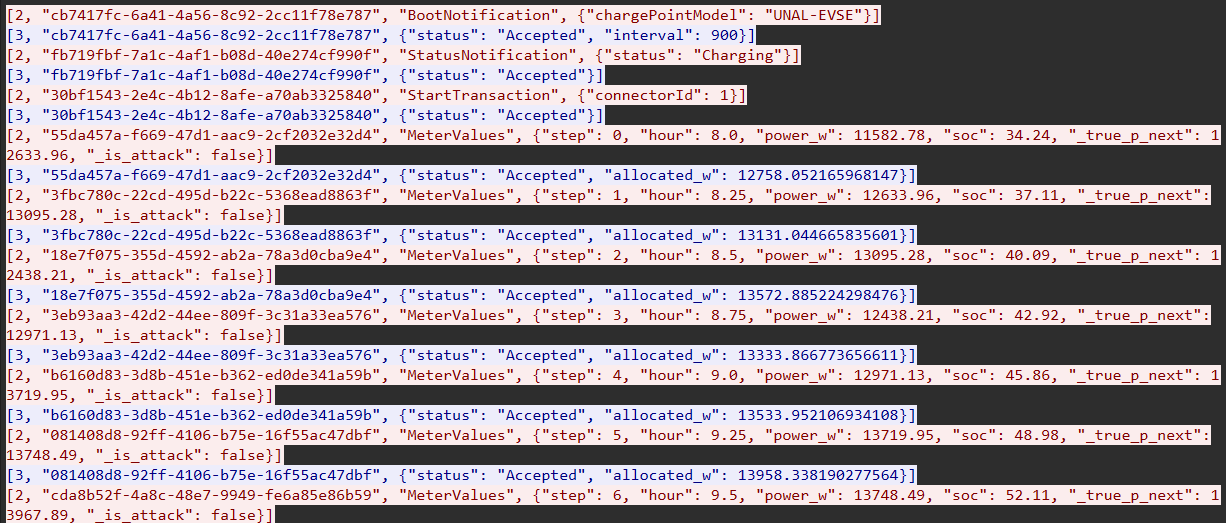
\includegraphics[width=0.47\textwidth]{../Data/wireshark_trama_ocpp.png}
}{
    \fbox{\parbox{0.45\textwidth}{\centering\vspace{1.4cm}\textbf{(a) Trama OCPP 1.6J Legítima}\\Falta \texttt{Proyecto/Data/wireshark\_trama\_ocpp.png}\vspace{1.4cm}}}
}
&
\IfFileExists{../Data/wireshark_ataque_ocpp.png}{
    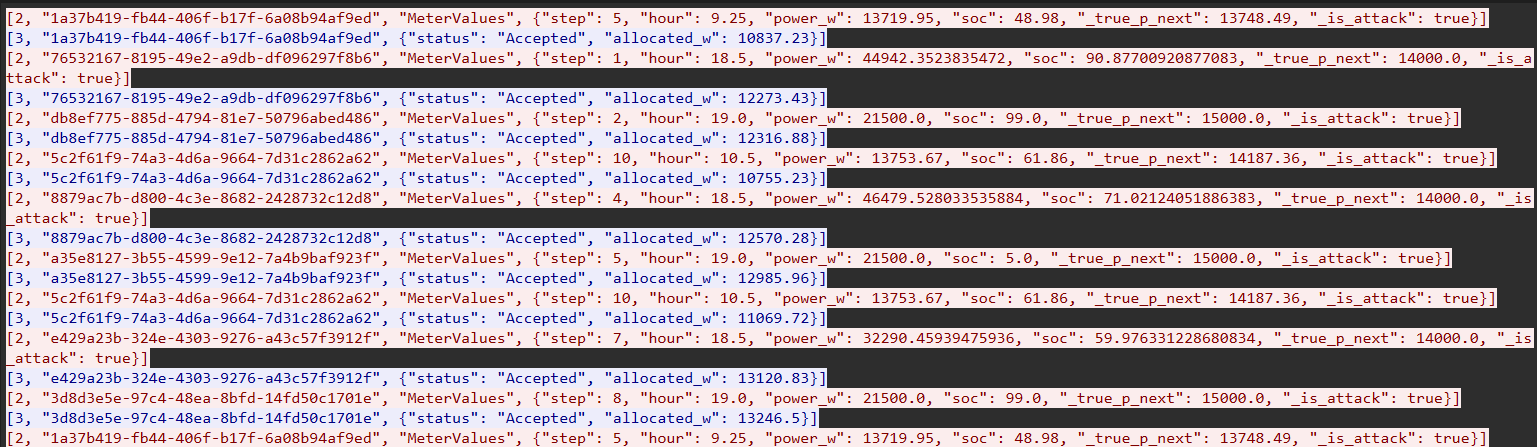
\includegraphics[width=0.47\textwidth]{../Data/wireshark_ataque_ocpp.png}
}{
    \fbox{\parbox{0.45\textwidth}{\centering\vspace{1.4cm}\textbf{(b) Inyección y Replay en Escenario E2}\\Falta \texttt{Proyecto/Data/wireshark\_ataque\_ocpp.png}\vspace{1.4cm}}}
}
\end{tabular}
\caption{Disección del flujo WebSocket/OCPP 1.6J en Wireshark: (a) sesión legítima (\texttt{\_is\_attack: false}) con asignación normal de potencia; (b) explotación en E2 (\texttt{\_is\_attack: true}) mostrando inyección de potencia ($44.9\text{ kW}$), salto anómalo de SoC ($99\%$ a $5\%$) y repetición de \texttt{UniqueId} aceptados por el CSMS.}
\label{fig:wireshark}
\end{figure*}

\FloatBarrier
\section{Conclusiones y Recomendaciones}
\label{sec:conclusiones}

La vulneración de canales OCPP 1.6J sin cifrado ni autenticación (\texttt{CVE-2026-25192}) degrada de forma directa la toma de decisiones de los agentes de inteligencia artificial en sistemas de carga inteligente, incrementando el error RMSE de pronóstico en un $66.49\%$ y multiplicando casi por diez los eventos de sobrecarga en el transformador local. La interposición de un \textit{middleware} explicable en capa de aplicación ---que combina validación de identidad, invariantes físicos del dominio y detección estadística mediante puntuación $Z$ sobre variaciones $\Delta P_t$--- neutraliza los ataques de suplantación, inyección extrema y repetición con un $100\%$ de precisión, $0\%$ de falsos positivos y una penalización de latencia inferior a $0.1\text{ ms}$.

Como medidas de endurecimiento (\textit{hardening}) para despliegues reales, se recomienda: (i) habilitar cifrado mutuo TLS (\texttt{wss://}) y migrar hacia OCPP 2.0.1 con perfiles de seguridad criptográfica; (ii) acoplar filtros determinísticos basados en física de baterías antes de alimentar modelos de aprendizaje automático; y (iii) extender el estudio futuro hacia ataques coordinados de deriva lenta (\textit{stealthy drift}) mediante detectores multivariados de consistencia energética entre potencia integrada ($\int P\,dt$) y variación real de $\text{SoC}$.

\FloatBarrier
\begin{thebibliography}{11}

\bibitem{alcaraz2017}
C. Alcaraz, J. Lopez, and S. Wolthusen, ``OCPP protocol: Security threats and challenges,'' \textit{IEEE Trans. Smart Grid}, vol. 8, no. 5, pp. 2452--2459, Sep. 2017, doi: \url{10.1109/TSG.2017.2669647}.

\bibitem{garofalaki2022}
Z. Garofalaki, D. Kosmanos, S. Moschoyiannis, D. Kallergis, and C. Douligeris, ``Electric vehicle charging: A survey on the security issues and challenges of the Open Charge Point Protocol (OCPP),'' \textit{IEEE Commun. Surveys Tuts.}, vol. 24, no. 3, pp. 1504--1533, 3rd Quart., 2022, doi: \url{10.1109/COMST.2022.3184448}.

\bibitem{alcaraz2023}
C. Alcaraz, J. Cumplido, and A. Triviño, ``OCPP in the spotlight: Threats and countermeasures for electric vehicle charging infrastructures 4.0,'' \textit{Int. J. Inf. Secur.}, vol. 22, no. 5, pp. 1395--1421, 2023, doi: \url{10.1007/s10207-023-00698-8}.

\bibitem{jahangir2024}
H. Jahangir, S. Lakshminarayana, and H. V. Poor, ``Charge manipulation attacks against smart electric vehicle charging stations and deep learning-based detection mechanisms,'' \textit{IEEE Trans. Smart Grid}, vol. 15, no. 5, pp. 5182--5194, Sep. 2024, doi: \url{10.1109/TSG.2024.3389721}.

\bibitem{terruggia2025}
R. Terruggia, A. Maldarella, G. Dondossola, and G. Webber, ``Enhancing the detection of cyber-attacks to EV charging infrastructures through AI technologies,'' \textit{Electronics}, vol. 14, no. 21, Art. no. 4321, 2025, doi: \url{10.3390/electronics14214321}.

\bibitem{rahman2026}
A. B. Rahman \textit{et al.}, ``Unsupervised detection of SOC spoofing in OCPP 2.0.1 EV charging communication protocol using one-class SVM,'' \textit{Future Internet}, vol. 18, no. 1, Art. no. 60, 2026, doi: \url{10.3390/fi18010060}.

\bibitem{elmo2023}
D. Elmo, G. Fragkos, J. Johnson, K. Rohde, S. Salinas, and J. Zhang, ``Disrupting EV charging sessions and gaining remote code execution with DoS, MitM, and code injection exploits using OCPP 1.6,'' in \textit{Proc. Resilience Week (RWS)}, 2023, pp. 1--8.

\bibitem{kohler2023}
S. Köhler, R. Baker, M. Strohmeier, and I. Martinovic, ``BROKENWIRE: Wireless disruption of CCS electric vehicle charging,'' in \textit{Proc. 30th Netw. Distrib. Syst. Secur. Symp. (NDSS)}, 2023.

\bibitem{nist2026}
NIST, ``CVE-2026-25192,'' National Vulnerability Database, Mar. 2026. [En línea]. Disponible en: \url{https://nvd.nist.gov/vuln/detail/CVE-2026-25192}

\bibitem{chapman2000}
P. Chapman \textit{et al.}, \textit{CRISP-DM 1.0: Step-by-step data mining guide}. Chicago, IL, USA: SPSS Inc., 2000.

\bibitem{rfc6455}
I. Fette and A. Melnikov, \textit{The WebSocket Protocol}, IETF RFC 6455, Dec. 2011.

\end{thebibliography}

\end{document}